\subsection{Сравнительный анализ параллельных численных алгоритмов решения уравнения квазиоптики}
\label{subsec:AppVs}

Как было сказано в \ref{sec:model}, для полного исследования явления филаментации необходимо решать уравнение квазиоптики на сетках
с количеством точек порядка $10^4$--$10^6$, а~значит потребность в оперативной памяти "--- величины около 4--100~Гб.
Это приводит к необходимости использования кластерных вычислительных систем и параллельных методов решения нелинейного уравнение квазиоптики.
Для определения области применимости двух описанных выше методов решения уравнения дифракции (на~основе преобразования Фурье и на основе разностной схемы)
были проведены тестовые замеры времени выполнения программы расчёта распространения пучка в среде с кубической  нелинейностью.
Цепочка уравнений, использованная в программе, имела следующий вид:

\begin{equation}\label{VarVsSplit}
    \left\{
    \begin{array}{rcl}
        2i\dfrac{\partial E}{\partial z} & = & \Delta_{\perp}E \\
        \\
        2i\dfrac{\partial E}{\partial z} & = & R\left|E\right|^2E
    \end{array}
    \right.
\end{equation}

Для выполнения быстрого преобразования Фурье использовалась свободно распространяемая библиотека FFTW (версии 2.3) \cite{FFTW}.
Подробнее c реализацией и методом создания алгоритма для FFTW можно ознакомиться в статьях \cite{FFTW1_98, FFTW2_Generator_99}.
Данная реализация БПФ предполагает ленточное распределение матрицы поля по процессам. Кроме того, FFTW, как любое быстрое преобразование Фурье,
эффективнее работает на~матрицах, размеры которых являются степенями двойки, поэтому для тестовых запусков использовались двумерные сетки
с количеством точек по одной координате $N = 512$, 1024, 2048, 4096, 8192, 16384. Для уменьшения влияния текущей загруженности кластера
и характеристик различных вычислительных узлов на результаты тестов замеры времени осуществлялись 10 раз в разное время суток и усреднялись.

Существенной особенностью алгоритмов БПФ является расположение полученных коэффициентов в памяти процессоров.
Для преобразования Фурье естественным является транспонированное расположение результата в памяти всех процессов.
Этому соответствует ключ \textsc{fftw\_transposed\_order} функции, реализующей преобразование Фурье.
Его альтернативой является ключ \textsc{fftw\_normal\_order}, при задании которого после выполнения преобразования Фурье
проводится дополнительное транспонирование матрицы спектра.
Кроме того существует параметр указанной функции, позволяющий использование дополнительного временного массива для ускорения преобразования.
Наконец, при создании плана Фурье-преобразования существует возможность оптимизировать план с целью ускорения работы функции.
Это достигается использованием ключей  \textsc{fftw\_estimate} (грубая оценка) и  \textsc{fftw\_measure} (при этом производятся замеры времени пересылок,
выполняемых в Фурье-преобразовании, и~их~оптимизация). Как показали тесты, для параллельной версии БПФ различие скорости расчётов
при использовании и без использования этого ключа отличаются в пределах статистической ошибки.

Ниже представлены результаты замеров времени работы алгоритма с использованием преобразования Фурье при различных комбинациях параметров,
выбранных для анализа их влияния на время работы программы на суперкомпьютере СКИФ МГУ <<Чебышёв>>.

    \newcommand{\minipagewidth}{0.45\linewidth}

    \begin{figure}[h!]
        \begin{center}
            \begin{minipage}{\minipagewidth}
                \center{Флаг \textsc{fftw\_estimate}:\\ \includegraphics[width=0.95\linewidth]{appendix_var_vs_fftw/skif/FFTW_compare_N512_nomeasure_2k}}
                \caption{Время работы Фурье-алгоритма в зависимости от количества процессов. Размер матрицы $512 \times 512$. }
                \label{fig:AppVsFourier512Nomeasure}
            \end{minipage}
            \hfill
            \begin{minipage}{\minipagewidth}
                \center{Флаг \textsc{fftw\_measure}:\\ \includegraphics[width=0.95\linewidth]{appendix_var_vs_fftw/skif/FFTW_compare_N512_measure_2k}}
                \caption{Время работы Фурье-алгоритма в зависимости от количества процессов. Размер матрицы $512 \times 512$.}
                \label{fig:AppVsFourier512Measure}
            \end{minipage}
        \end{center}
    \end{figure}

    \begin{figure}[h!]
        \begin{center}
            \begin{minipage}{\minipagewidth}
                \center{\includegraphics[width=0.95\linewidth]{appendix_var_vs_fftw/skif/FFTW_compare_N2048_nomeasure_2k}}
                \caption{Время работы Фурье-алгоритма в зависимости от количества процессов. Размер матрицы $2048 \times 2048$.}
                \label{fig:AppVsFourier2048Nomeasure}
            \end{minipage}
            \hfill
            \begin{minipage}{\minipagewidth}
                \center{\includegraphics[width=0.95\linewidth]{appendix_var_vs_fftw/skif/FFTW_compare_N2048_measure_2k}}
                \caption{Время работы Фурье-алгоритма в зависимости от количества процессов. Размер матрицы $2048 \times 2048$.}
                \label{fig:AppVsFourier2048Measure}
            \end{minipage}
        \end{center}
    \end{figure}

%%%%%%%%%%%%%%%%%%%%%%%%%%%%%%%%%%%%%%%%

    \newpage

    \begin{figure}[h!]
        \begin{center}
            \begin{minipage}{\minipagewidth}
                \center{Флаг \textsc{fftw\_estimate}:\\ \includegraphics[width=0.95\linewidth]{appendix_var_vs_fftw/skif/FFTW_compare_N8192_nomeasure_2k}}
                \caption{Время работы Фурье-алгоритма в зависимости от количества процессов. Размер матрицы $8192 \times 8192$.}
                \label{fig:AppVsFourier8192Nomeasure}
            \end{minipage}
            \hfill
            \begin{minipage}{\minipagewidth}
                \center{Флаг \textsc{fftw\_measure}:\\ \includegraphics[width=0.95\linewidth]{appendix_var_vs_fftw/skif/FFTW_compare_N8192_measure_2k}}
                \caption{Время работы Фурье-алгоритма в зависимости от количества процессов. Размер матрицы $8192 \times 8192$.}
                \label{fig:AppVsFourier8192Measure}
            \end{minipage}
        \end{center}
    \end{figure}

Из представленных на рис.~\ref{fig:AppVsFourier512Nomeasure},~\ref{fig:AppVsFourier512Measure} графиков видно, что использование более 8~процессоров является неэффективным для матрицы размером $512\times512$,
так как время работы программы возрастает по сравнению с временем работы программы при тех же параметрах на 8 процессорах.
Для размера матрицы $2048\times2048$, как видно из~рис.~\ref{fig:AppVsFourier2048Nomeasure},~\ref{fig:AppVsFourier2048Measure} увеличение числа процессоров дает ощутимое уменьшение времени работы программы.
При использовании матрицы размером $8192\times8192$ времена работы программы увеличиваются,
что позволяет более чётко увидеть различие во временах работы программы для различных комбинаций флагов при использовании библиотеки FFTW.


Из графиков на рис. \ref{fig:AppVsFourier512Nomeasure}--\ref{fig:AppVsFourier8192Measure} видно,
что использования флага \textsc{fftw\_measure} не приводит к~ускорению работы алгоритма.
Кроме того, использование буфера не~только не~привело к~ускорению алгоритма, но, наоборот, несколько затормозило его.
Скорость работы алгоритма с ключом \textsc{fftw\_transposed\_order}, как и ожидалось, оказалась выше, чем с ключом \textsc{fftw\_normal\_order}.


Далее были проведены замеры скорости выполнения программы для лучшего набора опций (отсутствие буфера, опции \textsc{fftw\_transposed\_order} и \textsc{fftw\_estimate}).
Замеры проводились без сохранения матрицы в файл и с параллельной записью матрицы в файл на каждом десятом шаге.
Рассчитанные по полученным данным ускорения и~эффективности программ представлены на рис. \ref{fig:AppVsSpeedupFourierNosave}--\ref{fig:AppVsEfficiencyFourierSave}.
Видно, что для размера матрицы поля, не превосходящего $2048\times2048$, использование более 8 процессов нецелесообразно.
Для больших матриц эффективность остаётся значительной: около 50\% от~идеальной для случая без сохранения данных и около 30\% для случая с сохранением.

Большие размеры матрицы и необходимость в дополнительной памяти для метода с использованием неявной схемы не позволили произвести расчёт с использованием одного процесса,
поэтому нормировка производилась на время работы программы на~4~процессах.

%%%%%%%%%%%%%%%%%%%%%%%%%%%%%%%%%%%%%%%%

    \newpage

    \begin{figure}[h!]
        \begin{center}
            \begin{minipage}{\minipagewidth}
                \center{\includegraphics[width=0.95\linewidth]{appendix_var_vs_fftw/skif/FFTW_time_nosave_all}} \\
                \caption{Время работы Фурье-алгоритма в зависимости от количества процессов. Сохранение данных в файл не производилось.}
                \label{fig:AppVsTimeFourierNosave}
            \end{minipage}
            \hfill
            \begin{minipage}{\minipagewidth}
                \center{\includegraphics[width=0.95\linewidth]{appendix_var_vs_fftw/skif/FFTW_time_withsave_all}} \\
                \caption{Время работы Фурье-алгоритма в зависимости от количества процессов. Сохранение данных в файл производилось на каждом десятом шаге.}
                \label{fig:AppVsTimeFourierSave}
            \end{minipage}
        \end{center}
    \end{figure}

    \begin{figure}[h!]
        \begin{center}
            \begin{minipage}{\minipagewidth}
                \center{\includegraphics[width=0.95\linewidth]{appendix_var_vs_fftw/skif/FFTW_acceleration_nosave_2k}} \\
                \caption{Ускорение Фурье-алгоритма в зависимости от количества процессов. Сохранение данных в файл не производилось.}
                \label{fig:AppVsSpeedupFourierNosave}
            \end{minipage}
            \hfill
            \begin{minipage}{\minipagewidth}
                \center{\includegraphics[width=0.95\linewidth]{appendix_var_vs_fftw/skif/FFTW_acceleration_withsave_2k}} \\
                \caption{Ускорение Фурье-алгоритма в зависимости от количества процессов. Сохранение данных в файл производилось на каждом десятом шаге.}
                \label{fig:AppVsSpeedupFourierSave}
            \end{minipage}
        \end{center}
    \end{figure}

    \begin{figure}[h!]
        \begin{center}
            \begin{minipage}{\minipagewidth}
                \center{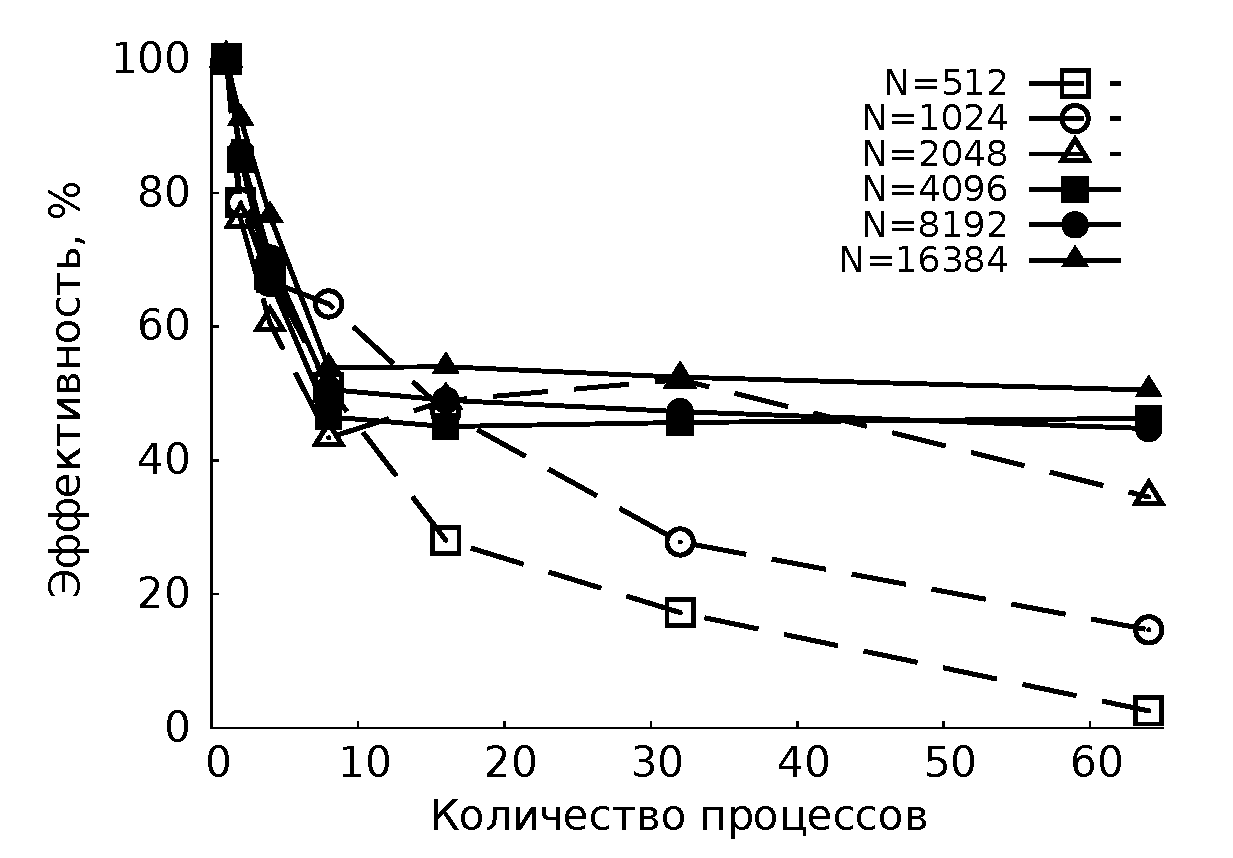
\includegraphics[width=0.95\linewidth]{appendix_var_vs_fftw/skif/FFTW_efficiency_nosave_2k}} \\
                \caption{Эффективность Фурье-алгоритма в зависимости от количества процессов. Сохранение данных в файл не производилось.}
                \label{fig:AppVsEfficiencyFourierNosave}
            \end{minipage}
            \hfill
            \begin{minipage}{\minipagewidth}
                \center{\includegraphics[width=0.95\linewidth]{appendix_var_vs_fftw/skif/FFTW_efficiency_withsave_2k}} \\
                \caption{Эффективность Фурье-алгоритма в зависимости от количества процессов. Сохранение данных в файл производилось на каждом десятом шаге.}
                \label{fig:AppVsEfficiencyFourierSave}
            \end{minipage}
        \end{center}
    \end{figure}

%%%%%%%%%%%%%%%%%%%%%%%%%%%%%%%%%%%%%%%%

    \newpage

    \begin{figure}[h!]
        \begin{center}
            \begin{minipage}{\minipagewidth}
                \center{
                    \includegraphics[width=0.95\linewidth]{appendix_var_vs_fftw/skif/Var_time_nosave_all}
                }
                \caption{Время работы алгоритма с неявной схемой в зависимости от количества процессов. Сохранение данных в файл не производилось.}
                \label{fig:AppVsTimeSkifNosave}
            \end{minipage}
            \hfill
            \begin{minipage}{\minipagewidth}
                \center{
                    \includegraphics[width=0.95\linewidth]{appendix_var_vs_fftw/skif/Var_time_withsave_all}
                }
                \caption{Время работы алгоритма с неявной схемой в зависимости от количества процессов. Сохранение данных в файл производилось на каждом десятом шаге.}
                \label{fig:AppVsTimeSkifSave}
            \end{minipage}
        \end{center}
    \end{figure}

    \begin{figure}[h!]
        \begin{center}
            \begin{minipage}{\minipagewidth}
                \center{
                    \includegraphics[width=0.95\linewidth]{appendix_var_vs_fftw/skif/Var_acceleration_nosave_all}
                }
                \caption{Ускорение алгоритма с неявной схемой в зависимости от количества процессов. Сохранение данных в файл не производилось.}
                \label{fig:AppVsSpeedupSkifNosave}
            \end{minipage}
            \hfill
            \begin{minipage}{\minipagewidth}
                \center{
                    \includegraphics[width=0.95\linewidth]{appendix_var_vs_fftw/skif/Var_acceleration_withsave_all}
                }
                \caption{Ускорение алгоритма с неявной схемой в зависимости от количества процессов. Сохранение данных в файл производилось на каждом десятом шаге.}
                \label{fig:AppVsSpeedupSkifSave}
            \end{minipage}
        \end{center}
    \end{figure}

    \begin{figure}[h!]
        \begin{center}
            \begin{minipage}{\minipagewidth}
                \center{
                    \includegraphics[width=0.95\linewidth]{appendix_var_vs_fftw/skif/Var_efficiency_nosave_all}
                }
                \caption{Эффективность алгоритма с неявной схемой в зависимости от количества процессов. Сохранение данных в файл не производилось.}
                \label{fig:AppVsEfficiencySkifNosave}
            \end{minipage}
            \hfill
            \begin{minipage}{\minipagewidth}
                \center{
                    \includegraphics[width=0.95\linewidth]{appendix_var_vs_fftw/skif/Var_efficiency_withsave_all}
                }
                \caption{Эффективность алгоритма с неявной схемой в зависимости от количества процессов. Сохранение данных в файл производилось на каждом десятом шаге.}
                \label{fig:AppVsEfficiencySkifSave}
            \end{minipage}
        \end{center}
    \end{figure}

%%%%%%%%%%%%%%%%%%%%%%%%%%%%%%%%%%%%%%%%

\newpage

Подведём итоги сравнения. В случае применения неявной разностной схемы требуется одна дополнительная матрица,
равная основной (она используется для хранения коэффициентов метода прогонки). Алгоритм показал отличную
масштабируемость, которая не сильно пострадала даже в случае периодического сохранения данных вычислений на диск.
При использовании метода на основе преобразования Фурье можно обойтись без использования дополнительной матрицы.
Но из-за более сложной организации пересылок при расчёте параллельного Фурье-преобразования
его масштабируемость ниже. Также наблюдается провал в производительности при небольших размерах матриц.


Таким образом, нельзя однозначно сказать, что какой-то какой метод всегда является лучшим.
В~случае, если задача не накладывает каких-то особых ограничений, лучше использовать метод на основе преобразования Фурье.
Если же имеется возможность использовать для расчёта очень большое число процессоров,
то целесообразно применения метода с неявной разностной схемой. Также этот метод будет применим
для задач с неравномерной сеткой по поперечному сечению, так как для них нет алгоритма
быстрого преобразования Фурье и метод с его использованием теряет свою актуальность.

